\newif\ifglobal

%%%%%%%%%%%%%%%%%%%%%%%
%%% Compile to view %%%
%%%%%%%%%%%%%%%%%%%%%%%

%%%%%%%%%%%%%%%%%%%%%%%%%%%%%%%%%%%%%%%%%%%%%%%%%%%
%%% Readme:                                     %%%
%%% https://www.overleaf.com/read/bwdjvfjksvjy/ %%%
%%%%%%%%%%%%%%%%%%%%%%%%%%%%%%%%%%%%%%%%%%%%%%%%%%%

% >>> M?: marks a module setting number or important notice

% >>> M4: Set {./relative-path} to external files for this module <<<
\def \modulefiles {./04-CAMLCDCTRL}
% To add an external file, use:
% (Replace '---' with actual filename)
% '\input{\modulefiles/tables/---.tex}' for tables
% '\includegraphics{\modulefiles/figures/---}' for figures
% '\subfile{\modulefiles/---}' for register files

% >>> M1: This module is in global project? <<<
% 'YES' - uncomment; 'NO' - comment out
\globaltrue

\ifglobal
    \documentclass[main\_\_EN.tex]{subfiles}

\else
    \documentclass[openany, 10pt]{book}

    % >>> M2: In ./00-shared/preamble-trm-module, also find
    %         settings for visibility of todo notes, watermark <<<
    \usepackage{preamble-trm-module}

    % >>> M3: Temporary labels in English,
    %         you can add your own labels there <<<
    \myexternaldocument{./00-shared/temp-labels-en}

\fi %\ifglobal


\setcounter{secnumdepth}{4}

% >>> M5: If this module needs any updates in
% './00-shared/preamble-trm-module.sty'
% (include additional package, etc.), contact your module PM
% or create the file './00-shared/changelog.tex' make the
% necessary updates yourself and document them in this file <<<


\begin{document}


% Sets language into which pre-defined bits of text are translated
\selectlanguage{english}

% Do not delete this block
\ifglobal
% Add the following front matter if
% this module is outside of global project
\else
    \InputIfFileExists{readme}{}{}
    {\let\clearpage\relax \listoftodos}
    \tableofcontents
    %\listoftables
    %\listoffigures
\fi


%%%%%%%%%%%%%%%%%%%%%%%%%
%%% TRM Module Begins %%%
%%%%%%%%%%%%%%%%%%%%%%%%%

\hypertarget{camlcdctrl}{}
\chapter{LCD and Camera Controller (LCD\_CAM)}
\label{mod:camlcdctrl}



\section{Overview}

This LCD and Camera (LCD\_CAM) controller consists of a LCD module and a camera module. The LCD module is designed to send parallel video data signals, and its bus supports RGB, MOTO6800, and I8080 interface timing. The camera module is designed to receive parallel video data signals, and its bus supports DVP 8-/16-bit modes.

\section{Features}

\begin{itemize}
    \item Supports the following operation modes:
    \begin{itemize}
        \item LCD master TX mode
        \item Camera slave RX mode
        \item Camera master RX mode
    \end{itemize}
    \item Supports simultaneous connection to an external LCD and an external camera
    \item When connected with an external LCD, the following is supported:
    \begin{itemize}
        \item 8-/16-bit parallel output mode
        \item RGB, MOTO6800, and I8080 LCD formats
        \item LCD data retrieved from internal memory via GDMA
    \end{itemize}
    \item When connected with an external camera (i.e., DVP image sensor), the following is supported:
    \begin{itemize}
        \item 8-/16-bit parallel input mode
        \item Camera data stored into internal memory via GDMA
    \end{itemize}
    \item Supports LCD\_CAM interface interrupts
\end{itemize}



\section{Functional Description}

\subsection{Block Diagram}
Figure  \ref{Figure:lcdcam_arch} shows the structure of this LCD\_CAM module, including
\begin{itemize}
    \item 1 x TX control unit (LCD\_Ctrl)
    \item 1 x RX control unit (Camera\_Ctrl)
    \item 1 x asynchronous TX FIFO (Async Tx FIFO) for communicating with external devices
    \item 1 x asynchronous RX FIFO (Async Rx FIFO) for communicating with external devices
    \item 2 x clock generators (LCD\_Clock Generator and CAM\_Clock Generator) for generating the module clocks
    \item 2 x format converters (RGB/YCbCr Converter) for converting video data into various formats
\end{itemize}


\begin{figure}[H]
    \centering
    \fbox{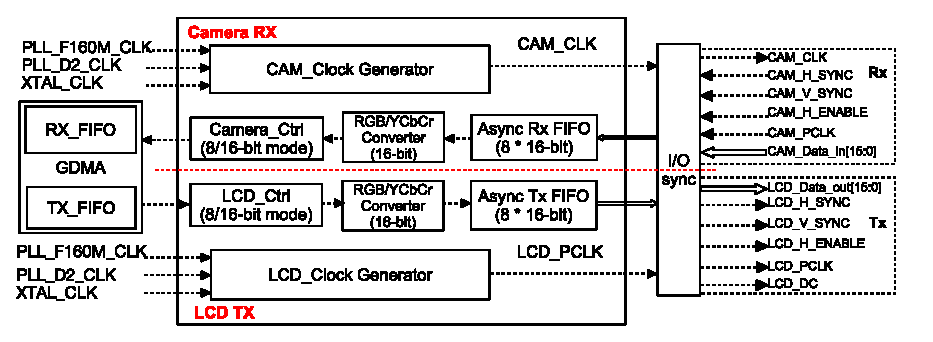
\includegraphics[width=1.0\textwidth]{04-CAMLCDCTRL/figures/i2s-arch_20220617.eps}}
     \textcolor{black}{\textbf{- ->}}: control signal
     \textcolor{black}{\textbf{=>}}: data flow
    \caption{LCD\_CAM Block Diagram}
    \label{Figure:lcdcam_arch}
\end{figure}




\subsection{Signal Description}



\begin{ThreePartTable}

\begin{TableNotes}
    \item[1] All signals of LCD\_CAM must be mapped to the chip's pin via GPIO matrix. For more information, see Chapter \ref{mod:iomuxgpio} \textit{\nameref{mod:iomuxgpio}}.
    \item[2] For the input/output signals with 8 or 16 bit width, \textcolor{red}{\it{N}} = 7 or 15 respectively.
    \item [3] If \hyperref[fielddesc:LCDCAMCAMVHDEMODEEN]{LCD\_CAM\_CAM\_VH\_DE\_MODE\_EN} is set, i.e., VSYNC + HSYNC mode is selected, in this mode, the signals of VSYNC, HSYNC and DE are used to control the data. For this case, users need to wire the three signal lines. If \hyperref[fielddesc:LCDCAMCAMVHDEMODEEN]{LCD\_CAM\_CAM\_VH\_DE\_MODE\_EN} is cleared, i.e., DE mode is selected, the signals of VSYNC and DE are used to control the data. For this case, wiring HSYNC signal line is not a must. But in this case, the YUV-RGB conversion function of camera module is not available.
\end{TableNotes}

\begin{longtable}[c]{ | l | l | c | p{8cm} | }
    \caption{Signal Description}
    \label{tab:signal-description}\\\hline

    \rowcolor{lightgray}
    \textbf{Operation Mode} & \textbf{Signal\tnote{1}} & \textbf{Direction} & \textbf{Function} \\\hline
    \endfirsthead

    \multicolumn{4}{c}{\bfseries \tablename\ \thetable{} -- cont'd from previous page}\\\hline
    \rowcolor{lightgray}
    \textbf{Operation Mode} & \textbf{Signal\tnote{1}} & \textbf{Direction} & \textbf{Function} \\\hline
    \endhead

    \multicolumn{4}{r}{\textbf{Cont'd on next page}} \\
    \endfoot

    \insertTableNotes
    \endlastfoot

    % table contents
    \multirow{5}*{Camera Slave RX Mode} & CAM\_PCLK & Input & Camera pixel clock signal \\\cline{2-4}
    & CAM\_V\_SYNC & Input& Vertical synchronization signal (VSYNC)\tnote{3}\\\cline{2-4}
    & CAM\_H\_SYNC & Input & Horizontal synchronization signal (HSYNC)\tnote{3}\\\cline{2-4}
    & CAM\_H\_ENABLE & Input & Horizontal enable signal (DE)\tnote{3}\\\cline{2-4}
    & CAM\_Data\_in[\textcolor{red}{\it{N}}:0]\tnote{2} & Input & Camera parallel input data bus, 8-/16-bit supported \\\hline
    \multirow{6}*{Camera Master RX Mode} & CAM\_PCLK & Input  & Camera pixel clock input signal\\\cline{2-4}
    & CAM\_CLK & Output& Camera master clock output signal \\\cline{2-4}
    & CAM\_V\_SYNC & Input& Vertical synchronization signal\tnote{3}\\\cline{2-4}
    & CAM\_H\_SYNC & Input & Horizontal synchronization signal\tnote{3}\\\cline{2-4}
    & CAM\_H\_ENABLE & Input & Horizontal enable signal\tnote{3} \\\cline{2-4}
    & CAM\_Data\_in[\textcolor{red}{\it{N}}:0]\tnote{2} & Input & Camera parallel input data bus, 8-/16-bit supported\\\hline
    \multirow{7}*{LCD Master TX Mode} & LCD\_PCLK & Output & LCD pixel clock signal \\\cline{2-4}
    & LCD\_H\_SYNC & Output & Horizontal synchronization signal in RGB format \\\cline{2-4}
    & LCD\_V\_SYNC & Output & Vertical synchronization signal in RGB mode  \\\cline{2-4}
    & LCD\_H\_ENABLE & Output & Horizontal enable signal in RGB format  \\\cline{2-4}
    & LCD\_CD & Output & Command and data (CD) signal in I8080 format\\\cline{2-4}
    & LCD\_CS & Output & Chip select (CS) signal in I8080/MOTO6800 format\\\cline{2-4}
    & LCD\_Data\_out[\textcolor{red}{\it{N}}:0]\tnote{2} & Output & LCD parallel output data bus, 8-/16-bit supported \\\hline
\end{longtable}

\end{ThreePartTable}



\subsection{LCD\_CAM Module Clocks}\label{sec:lcdcam-module-clk}

\subsubsection{LCD Clock}

The clocks used in LCD module are generated by LCD\_Clock Generator from clock sources, see Figure \ref{Figure:lcd_clk}.

The clocks include:
\begin{itemize}
    \item master clock: LCD\_CLK, divided from clock sources
    \item pixel clock: LCD\_PCLK, divided from LCD\_CLK
\end{itemize}

The clock source can be one of the following, depending on the configuration of \hyperref[fielddesc:LCDCAMLCDCLKSEL]{LCD\_CAM\_LCD\_CLK\_SEL} in register \hyperref[regdesc:LCDCAMLCDCLOCKREG]{LCD\_CAM\_LCD\_CLOCK\_REG}:
\begin{itemize}
    \item 0: disable LCD clock source
    \item 1: XTAL\_CLK
    \item 2: PLL\_D2\_CLK
    \item 3: PLL\_F160M\_CLK
\end{itemize}

\begin{figure}[H]
    \centering
    \fbox{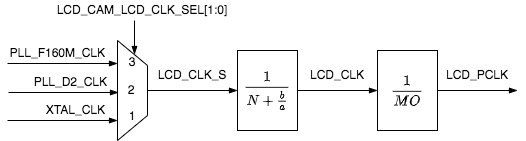
\includegraphics[width=0.8\textwidth]{04-CAMLCDCTRL/figures/lcd_clock_20220617.png}}
    \caption{LCD Clock}
    \label{Figure:lcd_clk}
\end{figure}

The following formula shows the relation between the frequency of LCD\_CLK ($f_{\textrm{LCD\_CLK}}$) and the divider clock source frequency ($f_{\textrm{LCD\_CLK\_S}}$):
$$f_{\textrm{LCD\_CLK}}=\frac{f_{\textrm{LCD\_CLK\_S}}}{\textrm{N} + \frac{\textrm{b}}{\textrm{a}}}$$

N is an integer value between 2 and 256. The value of N corresponds to the value of  \hyperref[fielddesc:LCDCAMLCDCLKMDIVNUM]{LCD\_CAM\_LCD\_CLKM\_DIV\_NUM} in register  \hyperref[regdesc:LCDCAMLCDCLOCKREG]{LCD\_CAM\_LCD\_CLOCK\_REG} as follows:

\begin{itemize}
    \item When  \hyperref[fielddesc:LCDCAMLCDCLKMDIVNUM]{LCD\_CAM\_LCD\_CLKM\_DIV\_NUM} = 0, N = 256.
    \item When  \hyperref[fielddesc:LCDCAMLCDCLKMDIVNUM]{LCD\_CAM\_LCD\_CLKM\_DIV\_NUM} = 1, N = 2.
    \item When  \hyperref[fielddesc:LCDCAMLCDCLKMDIVNUM]{LCD\_CAM\_LCD\_CLKM\_DIV\_NUM} has any other value, N = \hyperref[fielddesc:LCDCAMLCDCLKMDIVNUM]{LCD\_CAM\_LCD\_CLKM\_DIV\_NUM}.

\end{itemize}

``b" corresponds to the value of  \hyperref[fielddesc:LCDCAMLCDCLKMDIVB]{LCD\_CAM\_LCD\_CLKM\_DIV\_B}, and ``a" to the value of  \hyperref[fielddesc:LCDCAMLCDCLKMDIVA]{LCD\_CAM\_LCD\_CLKM\_DIV\_A}. For integer divider, \hyperref[fielddesc:LCDCAMLCDCLKMDIVA]{LCD\_CAM\_LCD\_CLKM\_DIV\_A} and  \hyperref[fielddesc:LCDCAMLCDCLKMDIVB]{LCD\_CAM\_LCD\_CLKM\_DIV\_B} are cleared. For fractional divider, the value of \hyperref[fielddesc:LCDCAMLCDCLKMDIVB]{LCD\_CAM\_LCD\_CLKM\_DIV\_B} should be less than the value of  \hyperref[fielddesc:LCDCAMLCDCLKMDIVA]{LCD\_CAM\_LCD\_CLKM\_DIV\_A}.


The following formula shows the relation between the frequencies of LCD\_PCLK ($f_{\textrm{LCD\_PCLK}}$ ) and LCD\_CLK ($f_{\textrm{LCD\_CLK}}$ ):

$$f_{\textrm{LCD\_PCLK}} = \frac{f_{\textrm{LCD\_CLK}}}{\textrm{MO}}$$


MO is determined by  \hyperref[fielddesc:LCDCAMLCDCLKEQUSYSCLK]{LCD\_CAM\_LCD\_CLK\_EQU\_SYSCLK} and  \hyperref[fielddesc:LCDCAMLCDCLKCNTN]{LCD\_CAM\_LCD\_CLKCNT\_N}.

\begin{itemize}
    \item When  \hyperref[fielddesc:LCDCAMLCDCLKEQUSYSCLK]{LCD\_CAM\_LCD\_CLK\_EQU\_SYSCLK} = 1, MO = 1.
    \item When  \hyperref[fielddesc:LCDCAMLCDCLKEQUSYSCLK]{LCD\_CAM\_LCD\_CLK\_EQU\_SYSCLK} = 0, MO = \hyperref[fielddesc:LCDCAMLCDCLKCNTN]{LCD\_CAM\_LCD\_CLKCNT\_N} + 1.
\end{itemize}

{\bfseries Notes: }
\begin{itemize}
    \item \hyperref[fielddesc:LCDCAMLCDCLKCNTN]{LCD\_CAM\_LCD\_CLKCNT\_N} must not be configured as 0.
    \item Using fractional divider may bring clock jitter. In case that LCD\_CLK and LCD\_PCLK can not be generated from PLL\_F160M\_CLK by integer divider, PLL\_D2\_CLK can be used as clock source. For more information, please refer to Chapter \ref{mod:resclk} \textit{\nameref{mod:resclk}}.
\end{itemize}

\subsubsection{Camera Clock}

The clocks used in camera module are generated by CAM\_Clock Generator from clock sources, see Figure \ref{Figure:camera_clk}.

The clocks include:
\begin{itemize}
    \item master clock: CAM\_CLK, master clock output from camera module, divided from clock sources.
    \item pixel clock: CAM\_CLK, clock input from camera slave.
\end{itemize}


\hyperref[fielddesc:LCDCAMCAMCLKSEL]{LCD\_CAM\_CAM\_CLK\_SEL} in register \hyperref[regdesc:LCDCAMCAMCTRLREG]{LCD\_CAM\_CAM\_CTRL\_REG} is used to select one of the following clock sources for camera module:
\begin{itemize}
    \item 0: disable camera clock source
    \item 1: XTAL\_CLK
    \item 2: PLL\_D2\_CLK
    \item 3: PLL\_F160M\_CLK
\end{itemize}


\begin{figure}[H]
    \centering
    \fbox{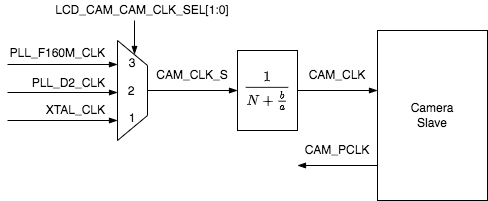
\includegraphics[width=0.8\textwidth]{04-CAMLCDCTRL/figures/camera_clock_20220617.png}}
    \caption{Camera Clock}
    \label{Figure:camera_clk}
\end{figure}

The following formula shows the relation between the frequencies of CAM\_CLK ($f_{\textrm{CAM\_CLK}}$ ) and the divider clock source ($f_{\textrm{CAM\_CLK\_S}}$ ):
$$f_{\textrm{CAM\_CLK}}=\frac{f_{\textrm{CAM\_CLK\_S}}}{\textrm{N} + \frac{\textrm{b}}{\textrm{a}}}$$

N is an integer value between 2 and 256. The value of N corresponds to the value of  \hyperref[fielddesc:LCDCAMCAMCLKMDIVNUM]{LCD\_CAM\_CAM\_CLKM\_DIV\_NUM} in register  \hyperref[regdesc:LCDCAMCAMCTRLREG]{LCD\_CAM\_CAM\_CTRL\_REG} as follows:

\begin{itemize}
    \item When  \hyperref[fielddesc:LCDCAMCAMCLKMDIVNUM]{LCD\_CAM\_CAM\_CLKM\_DIV\_NUM} = 0, N = 256.
    \item When  \hyperref[fielddesc:LCDCAMCAMCLKMDIVNUM]{LCD\_CAM\_CAM\_CLKM\_DIV\_NUM} = 1, N = 2.
    \item When  \hyperref[fielddesc:LCDCAMCAMCLKMDIVNUM]{LCD\_CAM\_CAM\_CLKM\_DIV\_NUM} has any other value, N = \hyperref[fielddesc:LCDCAMCAMCLKMDIVNUM]{LCD\_CAM\_CAM\_CLKM\_DIV\_NUM}.

\end{itemize}

``b" corresponds to the value of  \hyperref[fielddesc:LCDCAMCAMCLKMDIVB]{LCD\_CAM\_CAM\_CLKM\_DIV\_B}, and ``a" to the value of  \hyperref[fielddesc:LCDCAMCAMCLKMDIVA]{LCD\_CAM\_CAM\_CLKM\_DIV\_A}. For integer divider, \hyperref[fielddesc:LCDCAMCAMCLKMDIVA]{LCD\_CAM\_CAM\_CLKM\_DIV\_A} and  \hyperref[fielddesc:LCDCAMCAMCLKMDIVB]{LCD\_CAM\_CAM\_CLKM\_DIV\_B} are cleared. For fractional divider, the value of \hyperref[fielddesc:LCDCAMCAMCLKMDIVB]{LCD\_CAM\_CAM\_CLKM\_DIV\_B} should be less than the value of  \hyperref[fielddesc:LCDCAMCAMCLKMDIVA]{LCD\_CAM\_CAM\_CLKM\_DIV\_A}.



\subsection{LCD\_CAM Reset} \label{module_reset}
The units in LCD\_CAM module can be reset by the following bits:
\begin{itemize}
\item \hyperref[fielddesc:LCDCAMLCDRESET]{LCD\_CAM\_LCD\_RESET}: set this bit to reset LCD control unit (LCD\_Ctrl) and LCD video data format converter (RGB/YCbCr Converter).
\item \hyperref[fielddesc:LCDCAMCAMRESET]{LCD\_CAM\_CAM\_RESET}: set this bit to reset camera control unit (Camera\_Ctrl) and camera video data format converter (RGB/YCbCr Converter).
\item \hyperref[fielddesc:LCDCAMLCDAFIFORESET]{LCD\_CAM\_LCD\_AFIFO\_RESET}: set this bit to reset Async Tx FIFO.
\item \hyperref[fielddesc:LCDCAMCAMAFIFORESET]{LCD\_CAM\_CAM\_AFIFO\_RESET}: set this bit to reset Async Rx FIFO.
\end{itemize}


{\bfseries Notes: }
\begin{itemize}
    \item The above-mentioned reset bits are hardware self-clearing, i.e., the hardware automatically clears these bits once 1 is written.
    \item LCD/camera module clock must be configured first before the module and FIFO are reset.
\end{itemize}

\subsection{LCD\_CAM Data Format Control}
\subsubsection{LCD Data Format Control} \label{lcd_data_control}

When the LCD module is used to send data, the bit/byte order of the data from DMA can be adjusted by configuring

\begin{itemize}
    \item \hyperref[fielddesc:LCDCAMLCD2BYTEEN]{LCD\_CAM\_LCD\_2BYTE\_EN}
    \begin{itemize}
        \item 1: LCD output data is in 16-bit mode.
        \item 0: LCD output data is in 8-bit mode.
    \end{itemize}
    \item \hyperref[fielddesc:LCDCAMLCDBITORDER]{LCD\_CAM\_LCD\_BIT\_ORDER}
    \begin{itemize}
        \item 1: Change data bit order.
        \begin{itemize}
            \item Change LCD\_DATA\_out[7:0] to LCD\_DATA\_out[0:7] in 8-bit mode.
            \item Change LCD\_DATA\_out[15:0] to LCD\_DATA\_out[0:15] in 16-bit mode.
        \end{itemize}
        \item 0: Do not change the bit order.
    \end{itemize}
    \item \hyperref[fielddesc:LCDCAMLCDBYTEORDER]{LCD\_CAM\_LCD\_BYTE\_ORDER}
    \begin{itemize}
        \item 1: Invert data byte order, only valid in 16-bit mode.
        \item 0: Do not invert.
    \end{itemize}
    \item \hyperref[fielddesc:LCDCAMLCD8BITSORDER]{LCD\_CAM\_LCD\_8BITS\_ORDER}
    \begin{itemize}
        \item 1: Swap every two data bytes, valid in 8-bit mode
        \item 0: Do not swap.
    \end{itemize}
\end{itemize}
For the detailed configuration, see Table \ref{tab:bit-byte-order-control-of-lcd-data}.

\begin{table}[H]
    \centering
    \caption{LCD Data Format Control}
    \label{tab:bit-byte-order-control-of-lcd-data}
    \begin{threeparttable}
    \begin{tabular}{|p{2.3cm}|p{2.4cm}|p{2.5cm}|p{2.5cm}|p{2.6cm}|p{3.1cm}|}
    \hline
    \rowcolor{lightgray}
    \textbf{Data from DMA\tnote{1}} & \textbf{\hyperref[fielddesc:LCDCAMLCD2BYTEEN]{LCD\_CAM\_LCD\newline\_2BYTE\_EN}}  & \textbf{\hyperref[fielddesc:LCDCAMLCDBITORDER]{LCD\_CAM\_LCD\newline\_BIT\_ORDER}}  & \textbf{\hyperref[fielddesc:LCDCAMLCDBYTEORDER]{LCD\_CAM\_LCD\newline\_BYTE\_ORDER}\tnote{2}} &  \textbf{\hyperref[fielddesc:LCDCAMLCD8BITSORDER]{LCD\_CAM\_LCD\newline\_8BITS\_ORDER}\tnote{2}} & \textbf{TX Data\tnote{3,4}}
    \\ \hline
    \multirow{8}*{B0,B1,B2,B3} & \multirow{4}*{0} & \multirow{2}*{0} & 0 & 0 & \{B0\}\{B1\}\{B2\}\{B3\}     \\\cline{4-6}
                               &                  &                  & 0 & 1 & \{B1\}\{B0\}\{B3\}\{B2\}     \\\cline{3-6}
                               &                  & \multirow{2}*{1} & 0 & 0 & \{B0'\}\{B1'\}\{B2'\}\{B3'\} \\\cline{4-6}
                               &                  &                  & 0 & 1 & \{B1'\}\{B0'\}\{B3'\}\{B2'\} \\\cline{2-6}
                               & \multirow{4}*{1} & \multirow{2}*{0} & 0 & 0 & \{B1,B0\}\{B3,B2\}           \\\cline{4-6}
                               &                  &                  & 1 & 0 & \{B0,B1\}\{B2,B3\}           \\\cline{3-6}
                               &                  & \multirow{2}*{1} & 0 & 0 & \{B1',B0'\}\{B3',B2'\}       \\\cline{4-6}
                               &                  &                  & 1 & 0 & \{B0',B1'\}\{B2',B3'\}       \\\hline
    \end{tabular}
    \begin{tablenotes}
        \item[1] B0 \verb+~+ B3 represent the bytes of the data from DMA, from low address to high address.
        \item[2] Only the configuration listed in the table is valid. Other configuration may cause unexpected data errors.
        \item[3] In TX data, the bits in \{\} are in big-endian, and are in parallel with each other, while the data of \{\} is in serial with the data of other \{\}. Data is sent out from left to right. Take \{B0\}\{B1\}\{B2\}\{B3\} as an example. The bits in \{B0\} are in parallel with each other, but are in serial with the bits in \{B1\}\{B2\}\{B3\}. \{B0\} is sent out first.
        \item[4] In TX data, B{\textcolor{red}{n}}'[7:0] = B{\textcolor{red}{n}}[0:7] (n = 0,1,2,3).
    \end{tablenotes}
    \end{threeparttable}
\end{table}

\begin{tiplisting}
If only one byte of data is sent out each time, LCD\_Data\_out[7:0] is valid, while LCD\_Data\_out[15:8] is invalid.
\end{tiplisting}

\subsubsection{Camera Data Format Control} \label{cam_data_control}
When the camera module is used to receive data, the bit/byte order of the data to DMA can be adjusted by configuring
\begin{itemize}
    \item \hyperref[fielddesc:LCDCAMCAM2BYTEEN]{LCD\_CAM\_CAM\_2BYTE\_EN}
    \begin{itemize}
        \item 1: Camera input data is in 16-bit mode.
        \item 0: Camera input data is in 8-bit mode.
    \end{itemize}
    \item \hyperref[fielddesc:LCDCAMCAMBITORDER]{LCD\_CAM\_CAM\_BIT\_ORDER}
        \begin{itemize}
        \item 1: Change data bit order.
        \begin{itemize}
            \item Change CAM\_DATA\_in[7:0] to CAM\_DATA\_in[0:7] in 8-bit mode.
            \item Change CAM\_DATA\_in[15:0] to CAM\_DATA\_in[0:15] in 16-bit mode.
        \end{itemize}
        \item 0: Do not change the bit order.
    \end{itemize}
    \item \hyperref[fielddesc:LCDCAMCAMBYTEORDER]{LCD\_CAM\_CAM\_BYTE\_ORDER}
    \begin{itemize}
        \item 1: Invert data byte order, only valid in 16-bit mode.
        \item 0: Do not invert.
    \end{itemize}
\end{itemize}

For the detailed configuration, see Table \ref{tab:bit-byte-order-control-of-cam-data}.

\begin{table}[H]
    \centering
    \caption{CAM Data Format Control}
    \label{tab:bit-byte-order-control-of-cam-data}
    \begin{threeparttable}
    \begin{tabular}{|p{2.7cm}|p{2.6cm}|p{2.6cm}|p{2.6cm}|p{2.7cm}|}
    \hline
    \rowcolor{lightgray}
    \textbf{RX Data\tnote{1}} & \textbf{\hyperref[fielddesc:LCDCAMCAM2BYTEEN]{LCD\_CAM\_CAM\newline\_2BYTE\_EN}}  & \textbf{\hyperref[fielddesc:LCDCAMCAMBITORDER]{LCD\_CAM\_CAM\newline\_BIT\_ORDER}\tnote{2}}  & \textbf{\hyperref[fielddesc:LCDCAMCAMBYTEORDER]{LCD\_CAM\_CAM\newline\_BYTE\_ORDER}\tnote{2}} & \textbf{Data to DMA\tnote{3,4}}
    \\ \hline
    \multirow{2}*{\{B0\}\{B1\}\{B2\}\{B3\}} & \multirow{2}*{0} &        0         & 0 & B0,B1,B2,B3     \\\cline{3-5}
                                            &                  &        1         & 0 & B0',B1',B2',B3' \\\hline
    \multirow{4}*{\{B1,B0\}\{B3,B2\}}       & \multirow{4}*{1} & \multirow{2}*{0} & 0 & B0,B1,B2,B3     \\\cline{4-5}
                                            &                  &                  & 1 & B1,B0,B3,B2     \\\cline{3-5}
                                            &                  & \multirow{2}*{1} & 0 & B0',B1',B2',B3' \\\cline{4-5}
                                            &                  &                  & 1 & B1',B0',B3',B2' \\\hline
    \end{tabular}
    \begin{tablenotes}
        \item[1] In RX data, the bits in \{\} are in big-endian, and are in parallel with each other, while the data of \{\} is in serial with the data of other \{\}. Data is received from left to right. Take \{B0\}\{B1\}\{B2\}\{B3\} as an example. The bits in \{B0\} are in parallel with each other, but are in serial with the bits in \{B1\}\{B2\}\{B3\}. \{B0\} is received first.
        \item[2] Only the configuration listed in the table is valid. Other configuration may cause unexpected data errors.
        \item[3] B0 \verb+~+ B3 represent the bytes of the data to DMA, from low address to high address.
        \item[4] In the data to DMA, B{\textcolor{red}{n}}'[7:0] = B{\textcolor{red}{n}}[0:7] (n = 0,1,2,3).
    \end{tablenotes}
    \end{threeparttable}
\end{table}

\begin{tiplisting}
If only one byte is received each time, CAM\_Data\_in[7:0] is valid data. For such case, users must connect CAM\_Data\_in[7:0] with the master.
\end{tiplisting}

\subsection{YUV-RGB Data Format Conversion}
The LCD\_CAM module supports data format conversion among YUV and RGB. LCD module and camera module each has a data format converter. The converter supports format conversion over:
\begin{itemize}
    \item BT601 and BT709 standards
    \item RGB565 (full/limited range) and YUV422/420/411 (full/limited range) formats
    \item YUV422/420/411 (full/limited range) formats
\end{itemize}

\subsubsection{YUV Timing}
In LCD\_CAM module, assume that there are 8 pixels to be transmitted, corresponding to YUV data [$Y_i$, $U_i$, $V_i$] (i = 1 \verb+~+ 8). Then:
\begin{itemize}
    \item in YUV422 mode, the LCD sends (or the camera receives) the data as follows:
        \begin{table}[H]
            \centering
            \begin{tabular}{|c|c|c|c|c|c|c|c|c|c|c|c|c|c|c|c|}
            \hline
            $Y_1$ & $U_1$ & $Y_2$ & $V_2$ & $Y_3$ & $U_3$ & $Y_4$ & $V_4$ & $Y_5$ & $U_5$ & $Y_6$ & $V_6$ & $Y_7$ & $U_7$ & $Y_8$ & $V_8$ \\ \hline
            \end{tabular}
        \end{table}
    \item in YUV420 mode, the LCD sends (or the camera receives) the data as follows:
        \begin{table}[H]
            \centering
            \begin{tabular}{|c|c|c|c|c|c|c|c|c|c|c|c|}
            \hline
            $Y_1$ & $U_1$ & $Y_2$ & $Y_3$ & $U_3$ & $Y_4$ & $Y_5$ & $V_5$ & $Y_6$ & $Y_7$ & $V_7$ & $Y_8$ \\ \hline
            \end{tabular}
        \end{table}
    \item in YUV411 mode, the LCD sends (or the camera receives) the data as follows:
        \begin{table}[H]
            \centering
            \begin{tabular}{|c|c|c|c|c|c|c|c|c|c|c|c|}
            \hline
            $Y_1$ & $U_1$ & $Y_2$ & $Y_3$ & $V_3$ & $Y_4$ & $Y_5$ & $U_5$ & $Y_6$ & $Y_7$ & $V_7$ & $Y_8$ \\ \hline
            \end{tabular}
        \end{table}
\end{itemize}

\subsubsection{Data Conversion Configuration}
The configuration for format converter in camera module is identical to that in LCD module. Therefore, the configuration process is illustrated below using the format conversion in LCD module as an example:
\begin{itemize}
    \item Enable YUV-RGB format converter by setting  \hyperref[fielddesc:LCDCAMLCDCONVBYPASS]{LCD\_CAM\_LCD\_CONV\_BYPASS}.
    \item Configure the data transfer mode by configuring \hyperref[fielddesc:LCDCAMLCDCONVMODE8BITSON]{LCD\_CAM\_LCD\_CONV\_MODE\_8BITS\_ON}:
    \begin{itemize}
        \item 0: use 16-bit data transfer mode
        \item 1: use 8-bit data transfer mode
    \end{itemize}
    \item Select the standard by configuring \hyperref[fielddesc:LCDCAMLCDCONVPROTOCOLMODE]{LCD\_CAM\_LCD\_CONV\_PROTOCOL\_MODE}:
    \begin{itemize}
        \item 0: use BT601 standard
        \item 1: use BT709 standard
    \end{itemize}
    \item Configure the conversion mode:
    \begin{table}[H]
        \caption{Conversion Mode Control}
        \centering
        \begin{threeparttable}
        \begin{tabular}{|l|c|c|c|}
        \hline
        \rowcolor{lightgray}
        \textbf{Conversion Mode} & \textbf{\hyperref[fielddesc:LCDCAMLCDCONVTRANSMODE]{TRANS\_MODE}}\tnote{1} & \textbf{\hyperref[fielddesc:LCDCAMLCDCONVYUVMODE]{YUV\_MODE}}\tnote{2} & \textbf{\hyperref[fielddesc:LCDCAMLCDCONVYUV2YUVMODE]{YUV2YUV\_MODE}}\tnote{3} \\ \hline
        RGB565 -> YUV422 & 1 & 0 & 3 \\ \hline
        RGB565 -> YUV420 & 1 & 1 & 3 \\ \hline
        RGB565 -> YUV411 & 1 & 2 & 3 \\ \hline
        YUV422 -> RGB565 & 0 & 0 & 3 \\ \hline
        YUV420 -> RGB565 & 0 & 1 & 3 \\ \hline
        YUV411 -> RGB565 & 0 & 2 & 3 \\ \hline
        YUV422 -> YUV420 & 1 & 0 & 1 \\ \hline
        YUV422 -> YUV411 & 1 & 0 & 2 \\ \hline
        YUV420 -> YUV422 & 1 & 1 & 0 \\ \hline
        YUV420 -> YUV411 & 1 & 1 & 2 \\ \hline
        YUV411 -> YUV422 & 1 & 2 & 0 \\ \hline
        YUV411 -> YUV420 & 1 & 2 & 1 \\ \hline
        \end{tabular}
        \begin{tablenotes}
            \item[1] The value of  \hyperref[fielddesc:LCDCAMLCDCONVTRANSMODE]{LCD\_CAM\_LCD\_CONV\_TRANS\_MODE}
            \item[2] The value of  \hyperref[fielddesc:LCDCAMLCDCONVTRANSMODE]{LCD\_CAM\_LCD\_CONV\_YUV\_MODE}
            \item[3] The value of  \hyperref[fielddesc:LCDCAMLCDCONVTRANSMODE]{LCD\_CAM\_LCD\_CONV\_YUV2YUV\_MODE}
        \end{tablenotes}
     \end{threeparttable}
    \end{table}
    \item Configure the color range for input data by configuring \hyperref[fielddesc:LCDCAMLCDCONVDATAINMODE]{LCD\_CAM\_LCD\_CONV\_DATA\_IN\_MODE}:
    \begin{itemize}
        \item 1: full color range\hyperref[full-color-range-note]{$^1$}
        \item 0: limited color range\hyperref[limited-color-range-note]{$^2$}
    \end{itemize}
    \item Configure the color range for output data by configuring \hyperref[fielddesc:LCDCAMLCDCONVDATAOUTMODE]{LCD\_CAM\_LCD\_CONV\_DATA\_OUT\_MODE}:
    \begin{itemize}
        \item 0: limited color range
        \item 1: full color range
    \end{itemize}
\end{itemize}
\begin{tiplisting}
\vspace{-2em}
\begin{enumerate}
    \item \label{full-color-range-note} If full color range is selected, the color range of RGB or YUV is 0 \verb+~+ 255.
    \item \label{limited-color-range-note} If limited color range is selected,
    \begin{itemize}
    \item the color range of RGB is: 16 \verb+~+ 240.
    \item the color range of YUV is:
    \begin{itemize}
        \item Y: 16 \verb+~+ 240.
        \item U-V: 16 \verb+~+ 235.
    \end{itemize}
    \end{itemize}
\end{enumerate}
\end{tiplisting}

\section{Software Configuration Process}
\begin{tiplisting}
Updating the register configuration described in LCD module or camera module requires to set \hyperref[fielddesc:LCDCAMLCDUPDATE]{LCD\_CAM\_LCD\_UPDATE} and \hyperref[fielddesc:LCDCAMCAMUPDATE]{LCD\_CAM\_CAM\_UPDATE}, respectively, to synchronize registers from APB clock domain to LCD/camera clock domain. For more detailed configuration, see the configuration examples below.
\end{tiplisting}
\vspace{-2em}

\subsection{Configure LCD (RGB Format) as TX Mode}
Follow the steps below to configure LCD (RGB format) as TX mode via software:

\begin{enumerate}
    \item Configure clock according to Section \ref{sec:lcdcam-module-clk}.

    \item Configure signal pins according to Table \ref{tab:signal-description}.

    \item Enable corresponding interrupts, see Section \ref{LCDCAM_INT}.\label{LCDCAM-TX-INTERRUPT1}

    \item Enable RGB format by setting \hyperref[fielddesc:LCDCAMLCDRGBMODEEN]{LCD\_CAM\_LCD\_RGB\_MODE\_EN}.

    \item Configure frame format by the following registers. See the figures below.
    \begin{itemize}
        \item \hyperref[fielddesc:LCDCAMLCDVTHEIGHT]{LCD\_CAM\_LCD\_VT\_HEIGHT}
        \item \hyperref[fielddesc:LCDCAMLCDVTHEIGHT]{LCD\_CAM\_LCD\_VA\_HEIGHT}
        \item \hyperref[fielddesc:LCDCAMLCDVTHEIGHT]{LCD\_CAM\_LCD\_HB\_FRONT}
        \item \hyperref[fielddesc:LCDCAMLCDHTWIDTH]{LCD\_CAM\_LCD\_HT\_WIDTH}
        \item \hyperref[fielddesc:LCDCAMLCDHTWIDTH]{LCD\_CAM\_LCD\_HA\_WIDTH}
        \item \hyperref[fielddesc:LCDCAMLCDHTWIDTH]{LCD\_CAM\_VB\_FRONT}
        \item \hyperref[fielddesc:LCDCAMLCDVSYNCWIDTH]{LCD\_CAM\_LCD\_VSYNC\_WIDTH}
    \end{itemize}
    \begin{figure}[H]
    \centering
    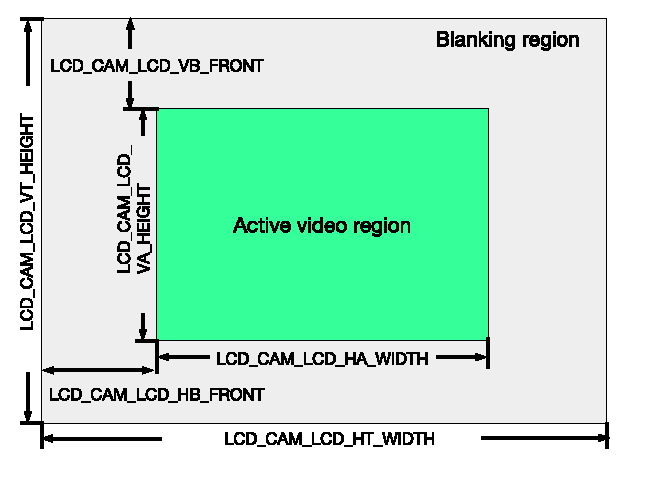
\includegraphics[width=0.6\textwidth]{04-CAMLCDCTRL/figures/lcd_frame_structure}
    \caption{LCD Frame Structure}
    \label{fig:lcd_frame}
\end{figure}

\begin{figure}[H]
    \centering
    \fbox{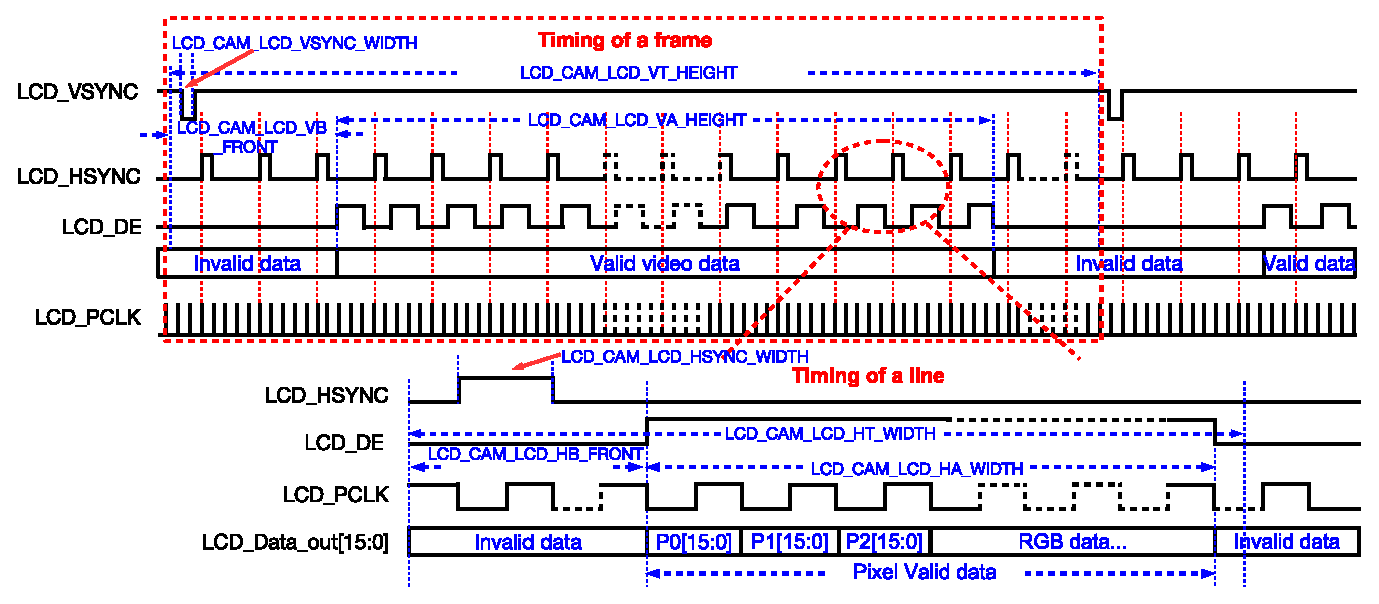
\includegraphics[width=1.0\textwidth]{04-CAMLCDCTRL/figures/lcd_timing_20220216}}
    \caption{LCD Timing (RGB Format)}
    \label{fig:lcd_timing}
\end{figure}
    \begin{tiplisting}
    When configuring the parameters shown in the figures above, please note that the parameter is equal to the register value + 1. For example, if the expected VSYNC width is 1, then please configure \hyperref[fielddesc:LCDCAMLCDVSYNCWIDTH]{LCD\_CAM\_LCD\_VSYNC\_WIDTH} to 0. For more information, see the register description.
\end{tiplisting}
    \item Set \hyperref[fielddesc:LCDCAMLCDUPDATE]{LCD\_CAM\_LCD\_UPDATE}.


    \item Reset TX control unit (LCD\_Ctrl) and Async Tx FIFO as described in Section \ref{module_reset}.

    \item Configure GDMA outlink.

    \item Start transmitting data:
    \begin{itemize}
        \item wait till LCD slave gets ready.
        \item then set \hyperref[fielddesc:LCDCAMLCDSTART]{LCD\_CAM\_LCD\_START} to start transmitting data.
    \end{itemize}


    \item Wait for the interrupt signals set in Step \ref{LCDCAM-TX-INTERRUPT1}.

    \item In frame intervals during data transmitting, check if the bit \hyperref[fielddesc:LCDCAMLCDNEXTFRAMEEN]{LCD\_CAM\_LCD\_NEXT\_FRAME\_EN} is set:
    \begin{itemize}
        \item If yes, set \hyperref[fielddesc:LCDCAMLCDUPDATE]{LCD\_CAM\_LCD\_UPDATE} (repeating the steps above) to continue transmitting next frame.
        \item If not, LCD stops transmitting data.
    \end{itemize}
    \item Clear \hyperref[fielddesc:LCDCAMLCDSTART]{LCD\_CAM\_LCD\_START} if data transmission is done.
\end{enumerate}

\subsection{Configure LCD (I8080/MOTO6800 Format) as TX Mode}

Figure \ref{fig:lcd_i8080_timing} shows the LCD timing sequence in I8080 format.


\begin{figure}[H]
    \centering
    \fbox{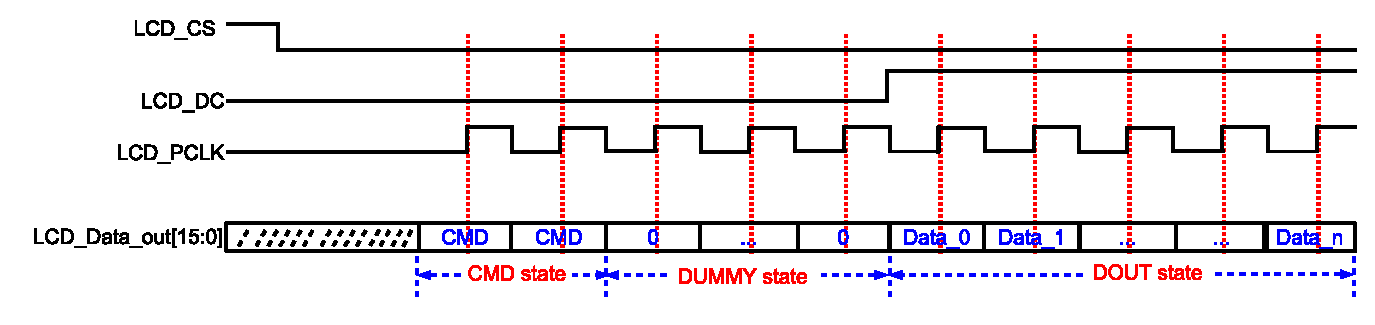
\includegraphics[width=1.0\textwidth]{04-CAMLCDCTRL/figures/LCD_I8080_Timg}}
    \caption{LCD Timing (I8080 Format)}
    \label{fig:lcd_i8080_timing}
\end{figure}

Follow the steps below to configure LCD (I8080 format) as TX mode via software:

\begin{enumerate}
    \item Configure clock according to Section \ref{sec:lcdcam-module-clk}.

    \item Configure signal pins according to Table \ref{tab:signal-description}.

    \item Enable corresponding interrupts, see Section \ref{LCDCAM_INT}.\label{LCDCAM-TX-INTERRUPT}

    \item Clear \hyperref[fielddesc:LCDCAMLCDRGBMODEEN]{LCD\_CAM\_LCD\_RGB\_MODE\_EN}.
    \item Configure CMD phase by \hyperref[fielddesc:LCDCAMLCDCMD]{LCD\_CAM\_LCD\_CMD}, \hyperref[fielddesc:LCDCAMLCDCMD2CYCLEEN]{LCD\_CAM\_LCD\_CMD\_2\_CYCLE\_EN}, and \hyperref[fielddesc:LCDCAMLCDCMDVALUE]{LCD\_CAM\\\_LCD\_CMD\_VALUE}.
    \item Configure DUMMY phase by \hyperref[fielddesc:LCDCAMLCDDUMMY]{LCD\_CAM\_LCD\_DUMMY} and \hyperref[fielddesc:LCDCAMLCDDUMMYCYCLELEN]{LCD\_CAM\_LCD\_DUMMY\_CYCLELEN}.
    \item Configure DOUT phase by \hyperref[fielddesc:LCDCAMLCDDOUT]{LCD\_CAM\_LCD\_DOUT}, depending on the output mode:
\begin{itemize}
    \item In a fixed-length output\hyperref[note-1]{$^a$}, configure data length in \hyperref[fielddesc:LCDCAMLCDDOUTCYCLELEN]{LCD\_CAM\_LCD\_DOUT\_CYCLELEN}.
    \item In a continuous output\hyperref[note-2]{$^b$}, set \hyperref[fielddesc:LCDCAMLCDALWAYSOUTEN]{LCD\_CAM\_LCD\_ALWAYS\_OUT\_EN}. Users do not need to configure \hyperref[fielddesc:LCDCAMLCDDOUTCYCLELEN]{LCD\_\\CAM\_LCD\_DOUT\_CYCLELEN}.
\begin{tiplisting}
\vspace{-2em}
\begin{enumerate}
    \item \label{note-1}
    In a fixed-length output, the LCD module stops sending data once the data length reaches the value set in \hyperref[fielddesc:LCDCAMLCDDOUTCYCLELEN]{LCD\_CAM\_LCD\_DOUT\_CYCLELEN}.
    \item \label{note-2} In a continuous output, LCD module keeps sending data till:
    \begin{enumerate}
        \item \hyperref[fielddesc:LCDCAMLCDSTART]{LCD\_CAM\_LCD\_START} is cleared;
        \item or \hyperref[fielddesc:LCDCAMLCDRESET]{LCD\_CAM\_LCD\_RESET} is set;
        \item or all the data in GDMA is sent out.
    \end{enumerate}
\end{enumerate}
\end{tiplisting}
\end{itemize}
    \item Configure the CD signal mode, including the default value of the CD signal and the values at each phase, see the description of \hyperref[regdesc:LCDCAMLCDMISCREG]{LCD\_CAM\_LCD\_MISC\_REG}.

    \item Set \hyperref[fielddesc:LCDCAMLCDUPDATE]{LCD\_CAM\_LCD\_UPDATE}.

    \item Reset TX control unit (LCD\_Ctrl) and Async Tx FIFO as described in Section \ref{module_reset}.

    \item Configure GDMA outlink.

    \item Start transmitting data:
    \begin{itemize}
        \item wait till LCD slave gets ready.
        \item then set \hyperref[fielddesc:LCDCAMLCDSTART]{LCD\_CAM\_LCD\_START} to start transmitting data.
    \end{itemize}


    \item Wait for the interrupt signals set in Step \ref{LCDCAM-TX-INTERRUPT}.

    \item Clear \hyperref[fielddesc:LCDCAMLCDSTART]{LCD\_CAM\_LCD\_START} if data transmission is done.
\end{enumerate}

\textbf{Notes:}\\
No matter in which format, RGB or I8080/MOTO6800, the rules below must be followed when accessing internal memory via GDMA:
\begin{itemize}
    \item If LCD data bus is configured to 8-bit parallel output mode, then
    \begin{itemize}
        \item pixel clock frequency must be less than 80 MHz.
        \item if YUV-RGB format conversion is used meanwhile, the pixel clock frequency must be less than 60 MHz.
    \end{itemize}
    \item If LCD data bus is configured to 16-bit parallel output mode, then
    \begin{itemize}
        \item pixel clock frequency must be less than 40 MHz.
        \item if YUV-RGB format conversion is used meanwhile, the pixel clock frequency must be less than 30 MHz.
    \end{itemize}
\end{itemize}

\subsection{Configure Camera as RX Mode}
Follow the steps below to configure camera as RX mode via software:

\begin{enumerate}
    \item Configure clock according to Section \ref{sec:lcdcam-module-clk}. Note that in slave mode, the module clock frequency should be two times faster than the PCLK frequency of the image sensor.

    \item Configure signal pins according to Table \ref{tab:signal-description}.

    \item Set or clear  \hyperref[fielddesc:LCDCAMCAMVHDEMODEEN]{LCD\_CAM\_CAM\_VH\_DE\_MODE\_EN} according to the control signal HSYNC.
    \item Set needed RX channel mode and RX data mode, then set the bit \hyperref[fielddesc:LCDCAMCAMUPDATE]{LCD\_CAM\_CAM\_UPDATE}.

    \item Reset RX control unit (Camera\_Ctrl) and Async Rx FIFO as described in Section \ref{module_reset}.
    \item Enable corresponding interrupts, see Section  \ref{LCDCAM_INT}.\label{LCDCAM-RX-INTERRUPT}

    \item Configure GDMA inlink, and set the length of RX data in \hyperref[fielddesc:LCDCAMCAMRECDATABYTELEN]{LCD\_CAM\_CAM\_REC\_DATA\_BYTELEN}.

    \item Start receiving data:
    \begin{itemize}
        \item In master mode, when the slave is ready, set \hyperref[fielddesc:LCDCAMCAMSTART]{LCD\_CAM\_CAM\_START} to start receiving data.
        \item In slave mode, set \hyperref[fielddesc:LCDCAMCAMSTART]{LCD\_CAM\_CAM\_START}. Receiving data starts after the master provides clock signal and control signal.
    \end{itemize}
    \item Receive data and store the data to the specified address of \chipname{} memory. Then corresponding interrupts set in Step \ref{LCDCAM-RX-INTERRUPT} will be generated.
\end{enumerate}

\textbf{Notes:}
\begin{itemize}
    \item No matter in which operation mode, camera master RX mode or camera slave RX mode, the rules below must be followed when accessing internal memory via GDMA:
\begin{itemize}

    \item If 8-bit parallel data input mode is selected, then
        \begin{itemize}
        \item pixel clock frequency must be less than 80 MHz.
        \item if YUV-RGB format conversion is used meanwhile, the pixel clock frequency must be less than 60 MHz.
    \end{itemize}
    \item If 16-bit parallel data input mode is selected, then
        \begin{itemize}
        \item pixel clock frequency must be less than 40 MHz.
        \item if YUV-RGB format conversion is used meanwhile, the pixel clock frequency must be less than 30 MHz.
    \end{itemize}
\end{itemize}
\item If an external camera and an external LCD are connected simultaneously, ensure that the maximum data throughput on the interface is less than GDMA total data bandwidth of 80 MB/s. Note the default frequency of APB\_CLK is 80 MHz here. For more information, see Chapter \ref{mod:resclk} \textit{\nameref{mod:resclk}}.
\end{itemize}

\section{LCD\_CAM Interrupts} \label{LCDCAM_INT}

\begin{itemize}
\item \label{int:LCDCAMCAMHSINT}LCD\_CAM\_CAM\_HS\_INT: triggered when the total number of received lines by camera is greater than or equal to \hyperref[fielddesc:LCDCAMCAMLINEINTNUM]{LCD\_CAM\_CAM\_LINE\_INT\_NUM} + 1.
\item \label{int:LCDCAMCAMVSYNCINT}LCD\_CAM\_CAM\_VSYNC\_INT: triggered when the camera received a VSYNC signal.
\item \label{int:LCDCAMLCDTRANSDONEINT}LCD\_CAM\_LCD\_TRANS\_DONE\_INT: triggered when the LCD transmitted all the data.
\item \label{int:LCDCAMLCDVSYNCINT}LCD\_CAM\_LCD\_VSYNC\_INT: triggered when the LCD transmitted a VSYNC signal.
\end{itemize}


% >>> If your module has no registers, delete sample text
%       for Sections Register Summary and Registers below <<<

%%%%%%%%%%%%%%%%%%%%%%%%
%%% Register Summary %%%
%%%%%%%%%%%%%%%%%%%%%%%%

% >>> Update the sample text below and insert
%     the info on register summary into the subfile <<<

\clearpage
\hypertarget{camlcdctrl-reg-summ}{}
\section{Register Summary}
\label{sec:camlcdctrl-reg-summ}

The addresses in this section are relative to LCD\_CAM controller base address provided in Table \ref{tab:sysmem-base-address} in Chapter \ref{mod:sysmem} \textit{\nameref{mod:sysmem}}.

The abbreviations given in Column \textbf{Access} are explained in Section \hyperref[glossary-access-types]{\textit{Access Types for Registers}}.

\subfile{\modulefiles/04-CAMLCDCTRL-reg-summ__EN}


%%%%%%%%%%%%%%%%%
%%% Registers %%%
%%%%%%%%%%%%%%%%%

% >>> Update the sample text below and insert
%      the info on registers into the subfile <<<

\clearpage
\section{Registers}

The addresses in this section are relative to LCD\_CAM controller base address provided in Table \ref{tab:sysmem-base-address} in Chapter \ref{mod:sysmem} \textit{\nameref{mod:sysmem}}.

\subfile{\modulefiles/04-CAMLCDCTRL-reg__EN}


\end{document}
